\chapter{Condiciones Operativas del Radio Transmisor}

El presente capítulo tiene como objetivo presentar el estudio realizado al radio transmisor, ya que para conocer su comportamiento térmico, se debía primero establecer que parámetros de funcionamiento tenían influencia en el comportamiento térmico del mismo, para luego caracterizar su comportamiento mediante un modelo que permitiera probar diferentes condiciones operativas y predecir su desempeño térmico. Para lo cual se sometió al radio a diferentes pruebas, con las cuales se pretendía obtener datos experimentales que permitieran conformar un modelo matemático a partir de dichos datos.

\section{Descripción General}

El radio transmisor en estudio es un KENWOOD modelo TM-D710A y sus principales características en valores nominales se muestran a continuación:\cite{manual}

\begin{table}[H]
    \centering
    \caption{\textbf{Características Eléctricas del Radio}}
    \begin{tabular}{cccc}
    \toprule
    \multicolumn{3}{c}{\textbf{Característica}} & \textbf{Magnitud}  \\
    \midrule
    \multicolumn{3}{c}{Voltaje} & \SI{13,8}{\volt} DC \num{\pm 15}\si{\percent} \\
    \midrule
    \multirow{6}{*}{Corriente} & \multirow{3}{*}{VHF} &  HI & Menor \SI{13}{\ampere} \\ && MID & Menor a \SI{5,5}{\ampere} \\ && LOW & Menor a \SI{4}{\ampere}\\
    & \multirow{3}{*}{UHF} &  HI & Menor a \SI{13}{\ampere}\\ && MID & Menor a \SI{6,5}{\ampere} \\ && LOW & Menor a \SI{5}{\ampere} \\
    \midrule
    \multicolumn{3}{c}{Rango de Temperatura de Operación} & De \SI{-20}{\celsius} a \SI{60}{\celsius}
    \\
    \midrule
    \multicolumn{2}{c}{\multirow{2}{*}{Masa (Aprox)}} & Panel de Operación & \SI{0,3}{\kilogram}\\
    && Unidad TX/RX & \SI{1,2}{\kilogram}\\
    \midrule
    \multicolumn{2}{c}{\multirow{3}{*}{Potencia de Salida RF}} & HI & \SI{50}{\watt}\\
    &&  MID & $\sim$\SI{10}{\watt} \\ && LOW & $\sim$\SI{5}{\watt} \\
    \bottomrule
    \end{tabular}
    \label{tab:1}
\end{table}

En la figura \ref{fotoradio} se observa que se trata de un radio transmisor de uso comercial, principalmente para transporte o automóviles, ya que el mismo cuenta con características como alertas del clima sin embargo, las mismas solo están disponibles en norteamerica. Es importante notar que el radio cuenta con tres partes externas principales: el micrófono, el panel frontal de control y la carcasa principal. Ni la imagen, ni lo antes descrito excluye el hecho de que para su correcto funcionamiento y dependiendo de la aplicación, el radio cuenta con otros elementos los cuales no se representan en la imagen.

\begin{figure}[H]
\centering
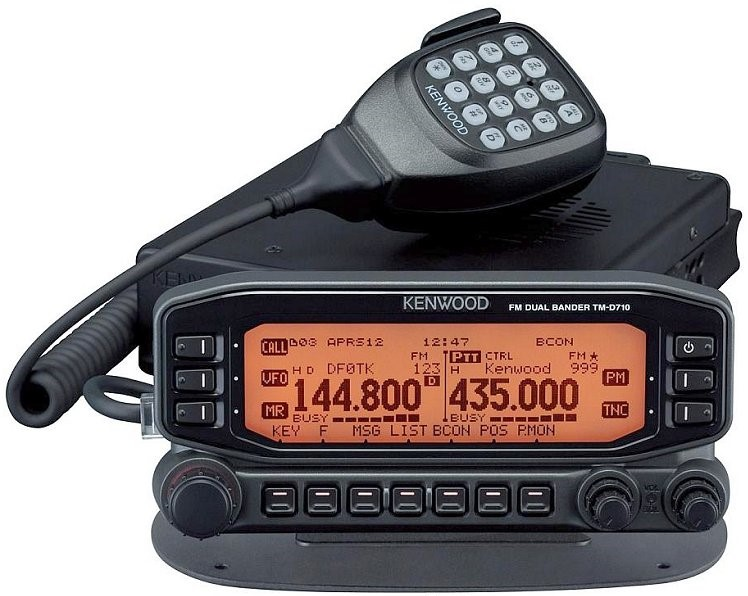
\includegraphics[scale=0.5]{Figuras/radio.jpg}
\caption{Radio KENWOOD TM-D710A}
Fuente:\cite{fotoradio}
\label{fotoradio}
\end{figure}

En síntesis, uno de los principales problemas, es implementar mecánica y térmicamente un radio de uso comercial, en un ambiente y aplicación no convencional o para lo cual no fue realmente diseñado; ya que de las partes antes descritas, es de especial interés, la carcasa principal, ya que la misma funciona como disipador térmico del radio, esto se convierte en un problema si la misma es retirada tal y como sucederá en la GRT, es decir, para lograr introducir el radio dentro de un gabinete en conjunto con otros elementos de la estación y optimizar el espacio, se debe desproveer el radio de todos aquellos elementos que no son estrictamente innecesarios. Para el caso particular de este radio el panel frontal de control no puede estar desconectado de la carcasa principal, ya que sin el radio no funciona, a pesar de que el mismo será operado remotamente; uno de los elementos que no estarán dentro de la estación es el micrófono que se observa en la Figura \ref{fotoradio}. 

\begin{figure}[H]
\centering
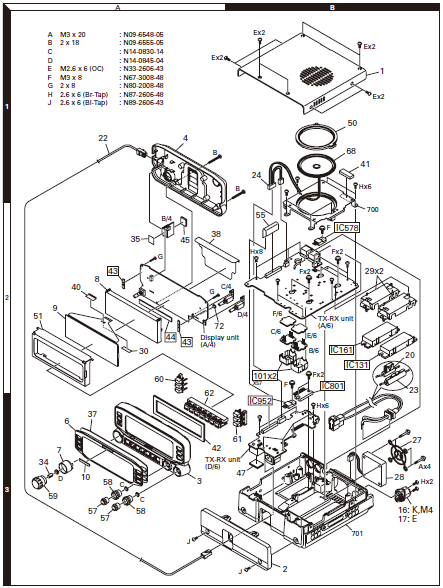
\includegraphics[scale=1.25]{Figuras/Despiece.png}
\caption{Despiece de Radio KENWOOD TM-D710A}
Fuente:\cite{manual}
\label{despiece}
\end{figure}

Como se observa en la Figura \ref{despiece}, el radio transmisor se trata de un dispositivo electrónico complejo, por lo que para realizar su análisis respectivo se consultó con los encargados del mismo y se llegó a las siguientes conclusiones preliminares:

\begin{itemize}
    \item El calor producido por el radio se concentra en el elemento TX-RX unit (A/6), lo que de ahora en adelante se conocerá como placa principal, y específicamente en los MOSFET de potencia marcados en la Figura \ref{despiece} como IC161 e IC131.
    \item El elemento descrito como TX-RX Unit (D/6), lo que de ahora en adelante se conocerá como placa secundaria se encuentra unida por dos puertos, uno de comunicación y otro de energía a la placa principal por lo cual dichos elementos no se pueden separar.
    \item El panel frontal de control deberá ir tal cual se muestra en en la Figura \ref{fotoradio} dentro del gabinete.
    \item El radio se despojará del micrófono y de elementos como el parlante (\#68) y los asociados al mismo.
    \item No se utilizarán en la estación de los elementos 1, 2 y 701 (Figura \ref{despiece}), de ahí es que surge la necesidad se implementar una solución mecánica para el soporte de la placa principal y secundaria.
\end{itemize}

\begin{figure}[H]
\centering
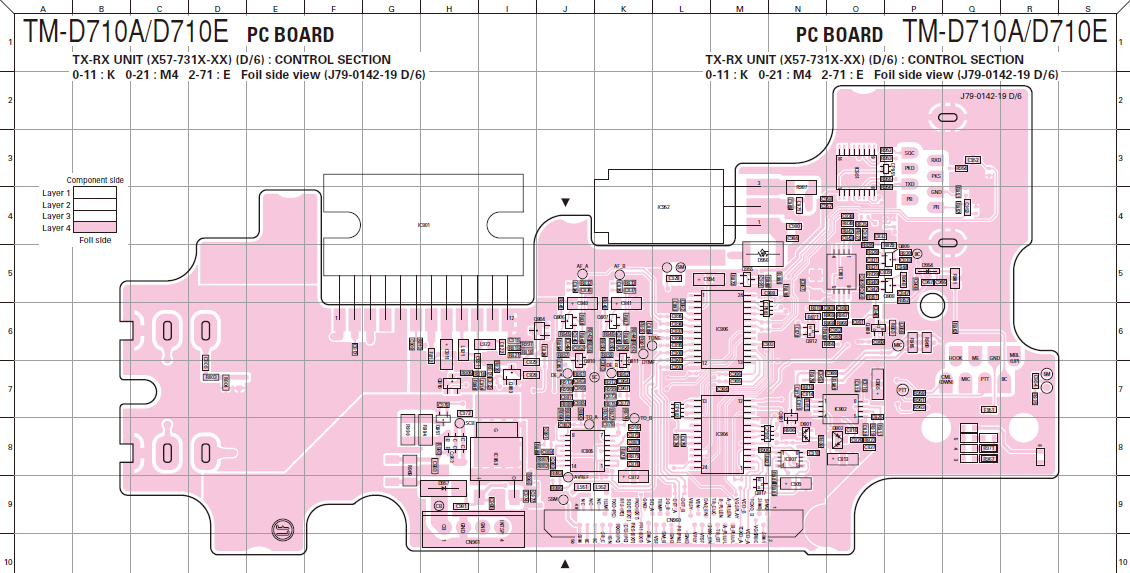
\includegraphics[scale=0.55]{Figuras/placasecundaria.png}
\caption{Plano de la PCB de la placa secundaria}
Fuente:\cite{manual}
\label{secundaria}
\end{figure}

\begin{figure}[H]
\centering
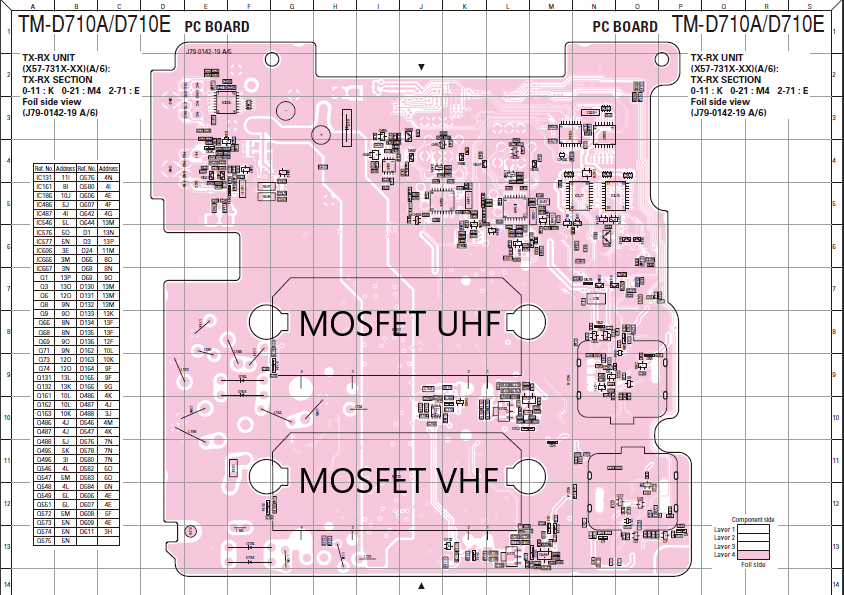
\includegraphics[scale=0.75]{Figuras/placaprincipal.png}
\caption{Plano de la PCB de la placa principal}
Fuente:\cite{manual}
\label{principal}
\end{figure}

En las Figuras \ref{secundaria} y \ref{principal} se presentan los planos de la tarjeta secundaria y principal respectivamente. En el caso de la placa principal se señala también los dos MOSFET de potencia que se identificaron como las fuentes de  calor a considerar, la más crítica el MOSFET de $UHF$, es el que mayor incremento de temperatura tendrá porque trabaja a una mayor frecuencia, además a pesar de tener dos canales de transmisión, simultáneamente solo se utilizará uno por lo tanto solo se estudiará el caso en el que la transmisión se realiza en $UHF$.

En cuanto al MOSFET de $UHF$ se tienen las siguientes características que se presentan en la Tabla \ref{mosfet}, de la cual cabe resaltar la temperatura de operación máxima que permite el dispositivo que junto con la temperatura máxima de operación del radio, establecen un parámetro que se debe cumplir dentro de la estación remota.  \cite{mosfet}

\begin{table}[H]
\centering
\caption{Características Generales del MOSFET de UHF}
\label{mosfet}
\begin{tabular}{lc}
\toprule
{\color[HTML]{000000} \textbf{Descripción}} & Silicon RF Power Modules \\
\textbf{Fabricante}                         & MITSUBISHI Electric      \\
\textbf{Número de parte}                    & RA60H4452M1              \\
\textbf{Código de Package}                  & H2M                      \\
\textbf{Rango de Frecuencia (\si{\mega\hertz})}          & 440-520                  \\
\textbf{Potencia Máxima (\si{\watt}})                & 60                       \\
\textbf{Voltaje de Alimentación (\si{\volt})}   & 12,5                     \\
\textbf{Temperatura de Operación (\si{\celsius})}      & -30 a 100                \\ \bottomrule
\end{tabular}
\end{table}

En el Apéndice \ref{anexo1} se muestra las características físicas del MOSFET de potencia, las cuales son características de un empaquetado tipo H2M.

\section{Adquisición de datos}

Como se mencionó en los antecedentes del proyecto, no existen registros históricos respecto al comportamiento tanto eléctrico como térmico del radio, tampoco información que corroborase que el aumento de temperatura provocaba la falla en el radio y por ende en la transmisión, ni datos concretos respecto a los parámetros de transmisión ni cuales de estos afectaban directamente al aumento de temperatura en el radio; es por eso que para realizar un modelo térmico del radio primero se requería obtener datos experimentales que permitieran relacionar el consumo energético con el aumento de temperatura. 

Para obtener los datos requeridos se utilizaron tres termocuplas tipo K, dos ``myDaq'' de la National Instruments, un sensor de corriente ASC712 y el software Labview 2017 para la implementación de la programación y almacenamiento de datos (Anexo \ref{anexo2},\ref{anexo3},\ref{anexo4},\ref{anexo5},\ref{anexo6}), en la Figura \ref{esquemaadquisicion} se muestra el esquema de implementación para la instrumentación. 

\begin{figure}[H]
\centering
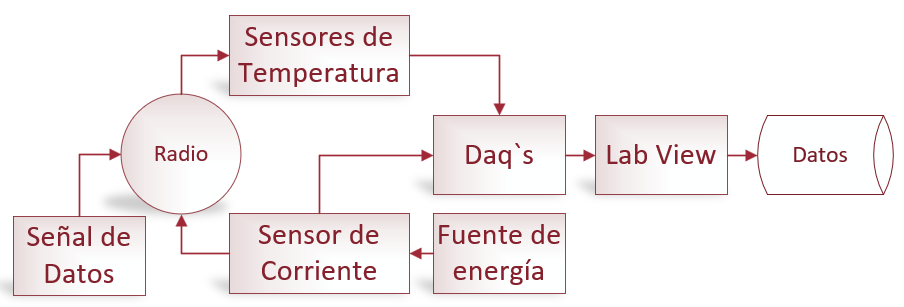
\includegraphics[scale=0.6]{Figuras/adquisicion.png}
\caption{Esquema de adquisición de datos}
Fuente: Elaboración Propia
\label{esquemaadquisicion}
\end{figure}

La hipótesis de experimentación se basa en que para lograr inducir una respuesta térmica en el radio se debe realizar un envió de paquetes de datos que simulen una transmisión, de manera tal que se correlacionen parámetros de transmisión, energía empleada y el aumento de temperatura lo cual no se logra con el baud rate o tasa de baudios la cual es de 1200 o 9600 propias de transmisiones en $VHF$ y $UHF$, está última se utilizará como parámetro fijo junto con la potencia de transmisión, ya que son valores que no tiene una variación durante el momento de la transmisión. Por otra parte se creía hasta este punto que el radio se apagaba durante las transmisiones debido a un circuito de protección térmica que desconectaba el mismo para evitar daños.

\subsection{Paquete de Datos}Esta constituido por líneas de información básica propia de la misión como la fecha, la hora en que se tomó la medición, datos de temperatura, humedad y nivel del humedal que se agrupan en un paquetes de líneas, en donde la cantidad de líneas es ajustable, ya que hasta el momento de las pruebas no se contaba con un tamaño de paquetes definido, sin embargo una línea no representa necesariamente el paquete de datos que envía el radio durante la transmisión, el mismo divide la información en lo que se conoce como tramas compuestas por un total de 276 Bytes máximo distribuidos de la siguiente manera:

\begin{table}[H]
\centering
\caption{Distribución de Bytes en una trama de información }
\label{trama}
\begin{tabular}{lc}
\toprule
\textbf{Sección}     & \textbf{Bytes} \\ \midrule
\textbf{Cabeceras}   & 2              \\
\textbf{Direcciones} & 14             \\
\textbf{Control}     & 1              \\
\textbf{PID}         & 1              \\
\textbf{Datos}       & 256            \\
\textbf{FCS}         & 2              \\ \bottomrule
\end{tabular}
\end{table}

Como se observa en la Tabla \ref{trama}, 18 de los 276 bytes son datos que acompañan a la información que se desea enviar; las cabeceras son un byte de información tanto al inicio como al final que indica cuando inicia un mensaje y cuando termina; las direcciones indican el destino de la información, luego se tiene un byte de control junto con uno de $PID$ o Identificador de paquete y dos bytes de $FCS$ o verificador de secuencia, el cual se encarga de corroborar la integridad de la información.


Es importante hacer la diferencia de que el baud rate no es lo mismo que el data rate o bit rate, es decir, las señales o símbolos por segundo no son iguales a los bits por segundo; la relación entre ellos esta definida por el esquema de modulación, que en este caso es el G3RUH, típico de sistemas en $VHF$ y $UHF$.

\subsection{Tiempo de transmisión} 

Depende directamente de la cantidad de líneas que contenga el paquete de datos; el radio una vez recibe la señal de transmitir abre el canal correspondiente y se mantiene enviando la información seccionada en tramas hasta que termine de enviar el paquete completo y cierre de nuevo el canal. Por otro lado se tiene el tiempo entre tramas que es el delay que puede o no existir entre las tramas o paquetes enviados.

\subsection{Parámetros de experimentación}\label{prueba}

Tomando en cuenta lo expuesto en las secciones anteriores, en la Figura \ref{diagrama_entrada_salida} se expone la propuesta de parámetros que se controlarán entre un experimento y otro, además de los datos que se esperan obtener al final de los experimentos.

\begin{figure}[H]
\centering
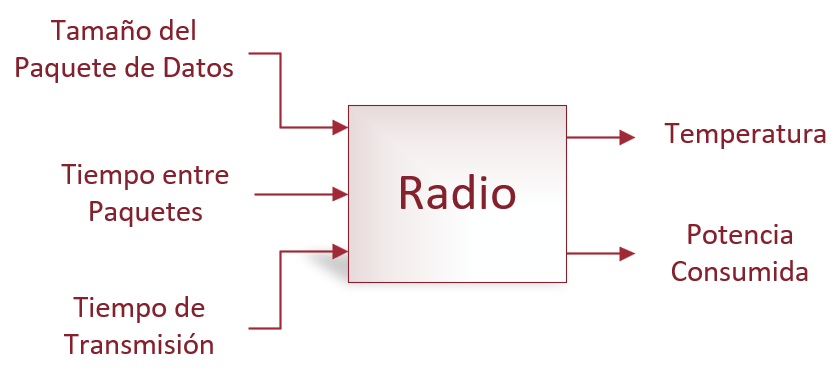
\includegraphics[scale=0.4]{Figuras/entradasalida.png}
\caption{Diagrama de Entradas y Salidas}
Fuente: Elaboración Propia
\label{diagrama_entrada_salida}
\end{figure}

Por otro lado  se dejaron como parámetros fijos en los experimentos:

\begin{table}[H]
\centering
\caption{Parámetros fijos de transmisión}
\label{fijos}
\begin{tabular}{lc}
\toprule
\textbf{Parámetro}           & \textbf{Valor} \\ \midrule
\textbf{Baud Rate (baudios)} & 9600           \\
\textbf{Frecuencia (\si{\mega\hertz})}    & 436            \\
\textbf{\begin{tabular}[c]{@{}l@{}}Potencia de\\ Transmisión (\si{\watt})\end{tabular}} & MID \\
\textbf{Canal}               & UHF            \\ \bottomrule
\end{tabular}
\end{table}

Todas las variables presentadas en la Tabla \ref{fijos} tiene relación de una forma u otra con el comportamiento térmico de radio, sin embargo al encontrarse relacionadas entre sí, un cambio en uno de estos parámetros podría implicar una variación en los demás, debido a que el baud rate está definido mediante un estándar que establece la frecuencia de la honda portadora de envió; a su vez las frecuencias están relacionadas con el canal, el cual implica un MOSFET en específico ya sea el de $VHF$ o el de $UHF$, es decir cada uno de los dos módulos de potencia (MOSFET) puede enviar o recibir datos dentro de un margen de frecuencias específico que no es el mismo entre ellos. Los encargados de realizar el enlace, determinaron que la potencia de transmisión  seleccionada era la suficiente para lograr transmitir los datos y para efectos de experimento se espera tener la condición que provoque mayor esfuerzo para el radio, lo cual en este caso sería en potencia media ya que de antemano se conocía que el radio se apagaba si se utilizaba en la máxima potencia; se retomará este tema cuando se realice el análisis de resultados. 

\section{Resultados obtenidos}

\subsection{Resultados Preliminares}

Previo a los experimentos formales, se realizaron pruebas preliminares, para determinar el comportamiento del radio, con el fin de establecer los valores de los parámetros en los experimentos de manera tal que se pudiera obtener la mayor cantidad de información posible, para lo cual se recurrió al micrófono del mismo, que de ahora en adelante se le conocerá como PTT (``Push to talk''); el cual permite simular una transmisión ya que tiene el mismo efecto sobre el módulo de potencia.

\begin{figure}[H]
\centering
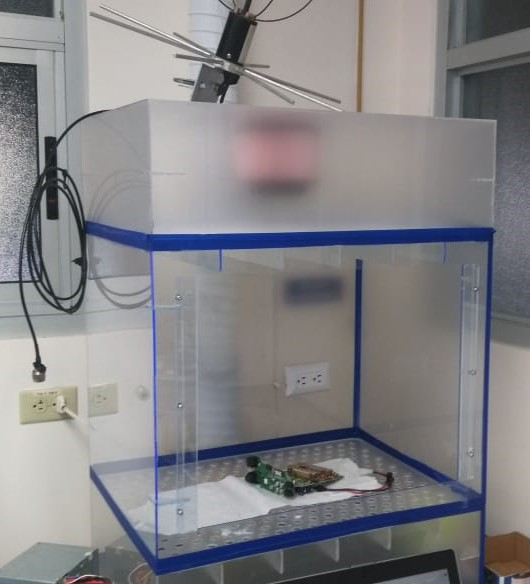
\includegraphics[scale=0.6]{Figuras/campana.jpeg}
\caption{Sitio de pruebas}
Fuente: Elaboración Propia
\label{campana}
\end{figure}


En la Figura \ref{campana} se muestran el lugar donde se colocó el radio, no se muestra todos los dispositivos utilizados para la realización de las pruebas. El recinto originalmente es utilizado para realizar montajes de dispositivos electrónicos bajo ambientes controlados (libre de polvo y partículas); la idea de realizar las pruebas en este sitio era la de eliminar en la medida de lo posible los efectos convectivos que son el resultado de corrientes de aire presentes en el laboratorio.

Para la prueba preliminar se utilizó el PTT en accionamientos que duraban 5 segundos aproximadamente y con un tiempo entre cada accionamiento de 5 segundos también, con intención de corroborar la hipótesis de que estos parámetros tienen un impacto en el comportamiento térmico significativo en el radio; la aproximación del tiempo se debe a que utilizar el PTT implica un proceso manual. Los resultados se muestran a continuación.

\begin{figure}[H]
\centering
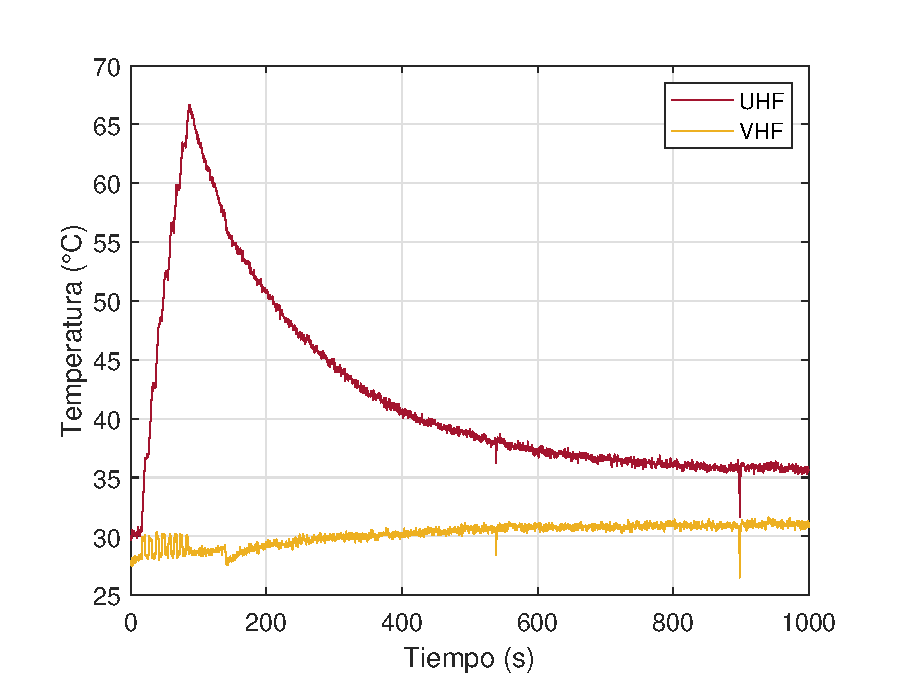
\includegraphics[scale=0.80]{Figuras/preliminar1.eps}
\caption{Gráfico Temperatura vs tiempo para los dos módulos de potencia}
Fuente: Elaboración Propia
\label{preliminar1}
\end{figure}

De la prueba realizada y de los datos mostrados en la Figura \ref{preliminar1} se obtienen la siguientes conclusiones y anotaciones:

\begin{itemize}
    \item Se confirma que durante la transmisión solo uno de los módulos de potencia permanece activo, el segundo presenta un leve incremento, mas no representativo y el cual podría está ligado a otras causas por lo que para efectos de las siguientes pruebas todos los datos mencionados hacen referencia al módulo de potencia de $UHF$.
    \item El incremento de temperatura presenta un comportamiento con una pendiente  elevada, lo cual confirma la necesidad térmica planteada y a su vez, que los parámetros de experimentación seleccionados, son representativos y al controlarlos se pueden obtener diferentes comportamientos térmicos.
    \item El rápido incremento en la temperatura pone de manifiesto la advertencia de no exceder los valores de temperatura de operación de los módulos de potencia, por el daño y degradación que los mismos podrían sufrir,esto implica que el tiempo de transmisión se vuelve relevante tanto para los experimentos como para la operación dentro de la estación remota. 
    \item El tiempo aproximado de transmisión fue de 2 minutos, sin embargo bajo condiciones de convección natural disminuidas el radio tarda aproximadamente 15 minutos en alcanzar una temperatura estable, pero aún así por encima de la inicial.
    
\end{itemize}

\subsection{Experimentos planteados}

Se plantearon 4 experimentos formales de los cuales se obtuvo información para realizar el modelo matemático del radio y poder realizar comparaciones.

\begin{table}[H]
\centering
\caption{Parámetros de entrada en los experimentos}
\label{parametros_experimento}
\begin{tabular}{lcccc}
\toprule
\multicolumn{1}{c}{\multirow{2}{*}{\textbf{Parámetro}}} & \multicolumn{4}{c}{\textbf{Experimento}}                                                              \\ \cline{2-5} 
\multicolumn{1}{c}{}        & \textbf{1} & \textbf{2} & \textbf{3} & \textbf{4} \\ \midrule
Tamaño de paquete (Bytes)                               & \multicolumn{1}{l}{4000} & \multicolumn{1}{l}{4000} & \multicolumn{1}{l}{42} & \multicolumn{1}{l}{42} \\ 
Tiempo de transmisión (\si{\min}) & 4:57       & 4:51       & 1          & 1          \\
Tiempo entre paquetes (\si{\second})     & 8         & 10          & 1          & 5          \\
Voltaje Real (\si{\volt}) & \multicolumn{4}{c}{12.12}\\
Temperatura ambiente (\si{\celsius}) & \multicolumn{4}{c}{24}\\ 
\bottomrule
\end{tabular}
\end{table}

En cuanto al tamaño del paquete los primeros dos experimentos se realizaron con un archivo de datos de prueba que se utilizaba para comprobar la programación de la transmisión para el caso de los experimentos 3 y 4 se ajustó el tamaño del paquete al de una línea de información. Los tiempos de transmisión se determinaron según las predicciones realizadas por el laboratorio de los tiempos de pasadas óptimas, es decir, el tiempo durante el cual el satélite pasa dentro de un rango de área que permite el enlace satelital con el radio de la estación remota, mientras el mismo orbita sobre la tierra. Los estudios indicaron que para la órbita del satélite y las condiciones geográficas de Palo Verde las pasadas promedio tienen una duración aproximada de 5 minutos, mientras que el tiempo mínimo de una pasada ronda el minuto. Por último, el tiempo entre paquetes se determinó basado en la experiencia de las pruebas preliminares.

\subsection{Datos obtenidos}

A continuación se muestran los resultados obtenidos de los cuatro experimentos:

\textbf{Experimento 1:}

\begin{figure}[H]
\centering
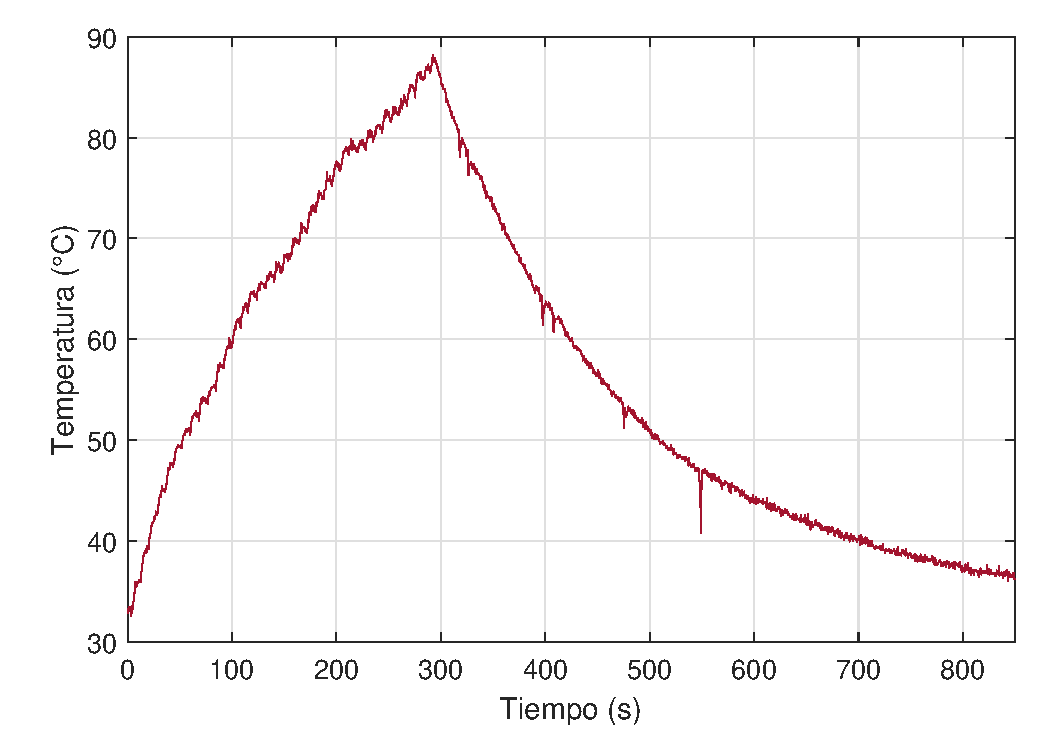
\includegraphics[scale=0.65]{Figuras/Exp2_T.eps}
\caption{Gráfico Temperatura vs tiempo para el Experimento 1}
Fuente: Elaboración Propia
\label{exp1_T}
\end{figure}

\begin{figure}[H]
\centering
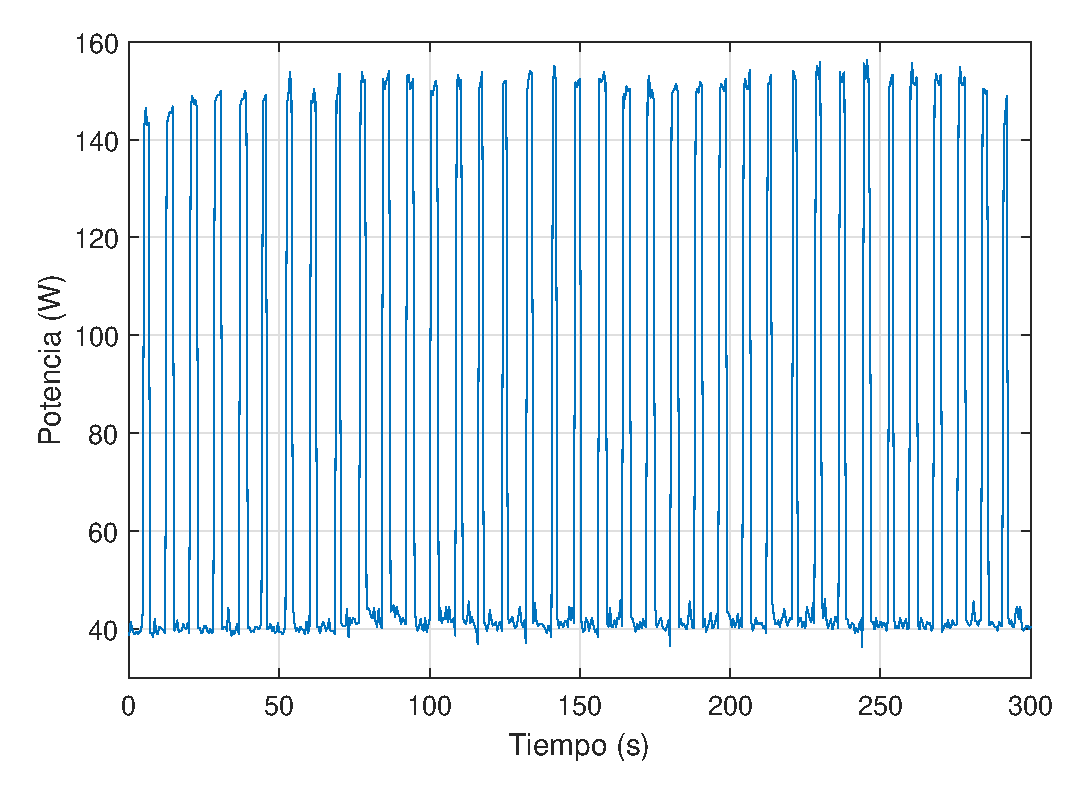
\includegraphics[scale=0.65]{Figuras/Exp2_P.eps}
\caption{Gráfico Potencia vs tiempo para el Experimento 1}
Fuente: Elaboración Propia
\label{exp1_P}
\end{figure}

\textbf{Experimento 2:}

\begin{figure}[H]
\centering
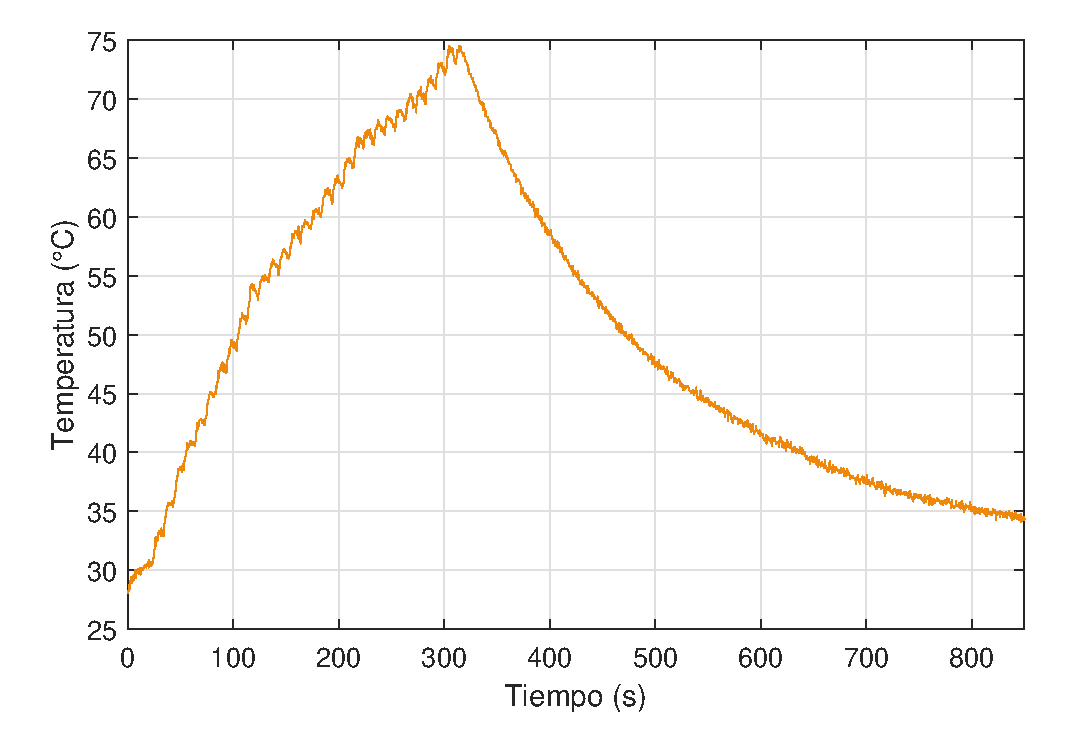
\includegraphics[scale=0.64]{Figuras/Exp1_T.eps}
\caption{Gráfico Temperatura vs tiempo para el Experimento 2}
Fuente: Elaboración Propia
\label{exp2_T}
\end{figure}

\begin{figure}[H]
\centering
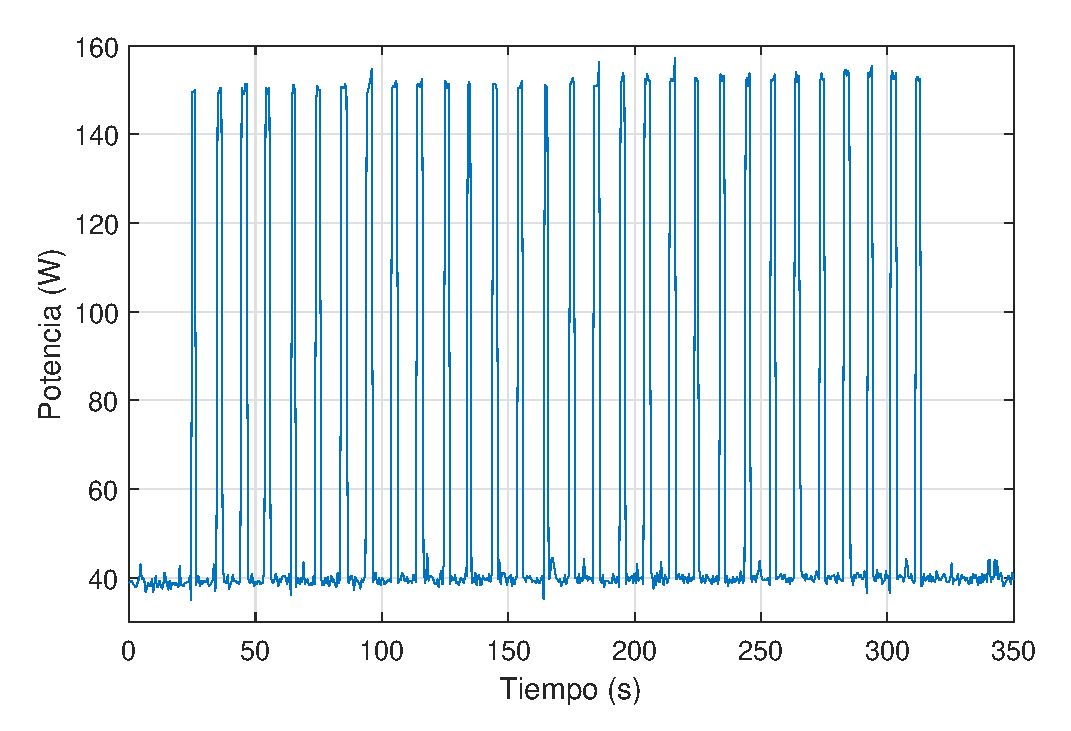
\includegraphics[scale=0.66]{Figuras/Exp1_P.eps}
\caption{Gráfico Potencia vs tiempo para el Experimento 2}
Fuente: Elaboración Propia
\label{exp2_P}
\end{figure}
%Tuve un error en el orden los experimentos al guardar los graficos por eso el nombre de las figuras esta invertido
\textbf{Experimento 3:}

\begin{figure}[H]
\centering
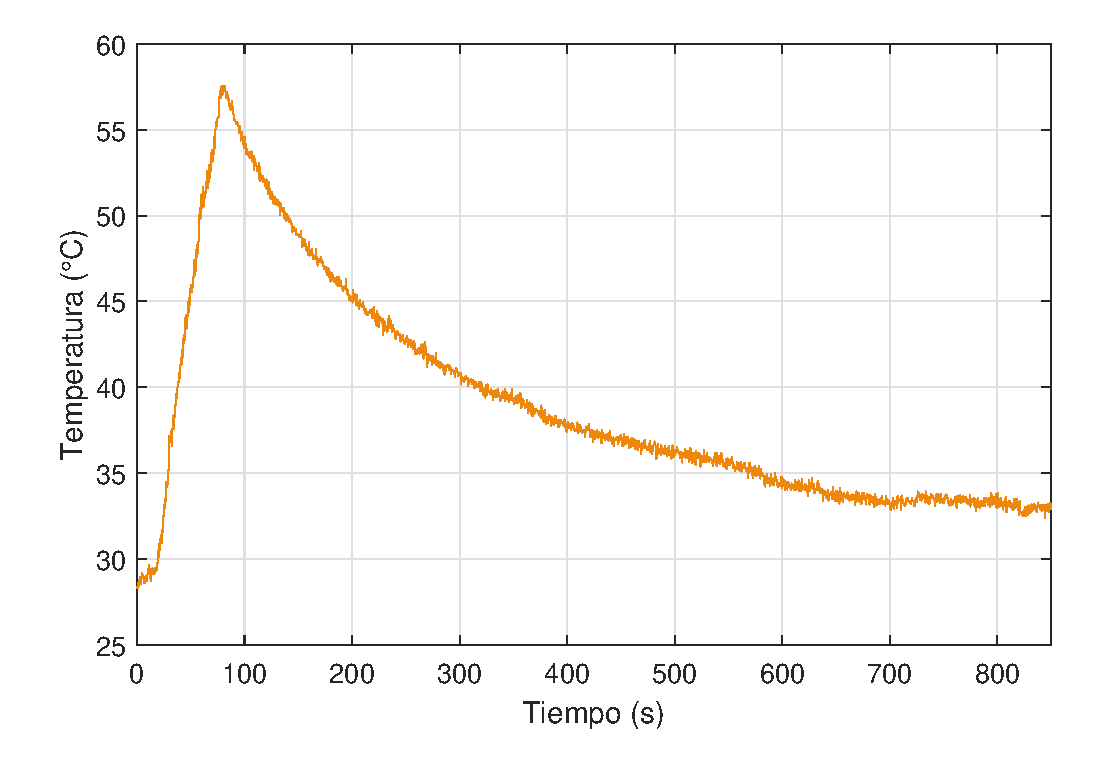
\includegraphics[scale=0.65]{Figuras/Exp4_T.eps}
\caption{Gráfico Temperatura vs tiempo para el Experimento 3}
Fuente: Elaboración Propia
\label{exp4_T}
\end{figure}

\begin{figure}[H]
\centering
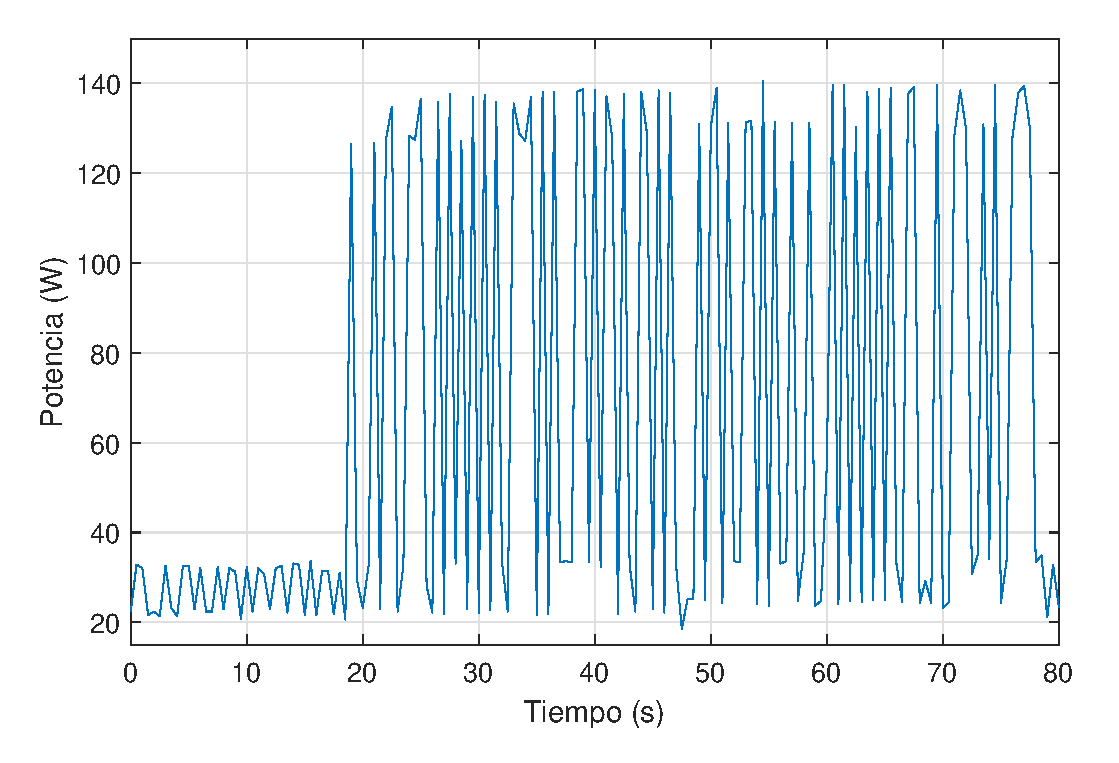
\includegraphics[scale=0.66]{Figuras/Exp4_P.eps}
\caption{Gráfico Potencia vs tiempo para el Experimento 3}
Fuente: Elaboración Propia
\label{exp4_P}
\end{figure}

\textbf{Experimento 4:}

\begin{figure}[H]
\centering
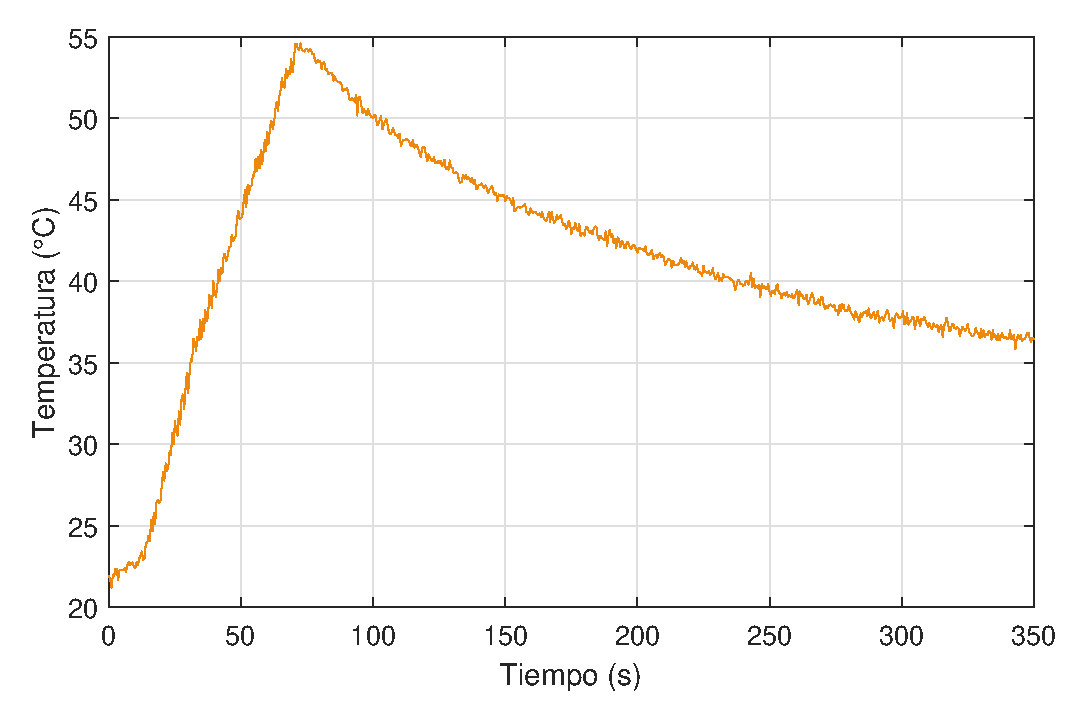
\includegraphics[scale=0.65]{Figuras/Exp3_T.eps}
\caption{Gráfico Temperatura vs tiempo para el Experimento 4}
Fuente: Elaboración Propia
\label{exp3_T}
\end{figure}

\begin{figure}[H]
\centering
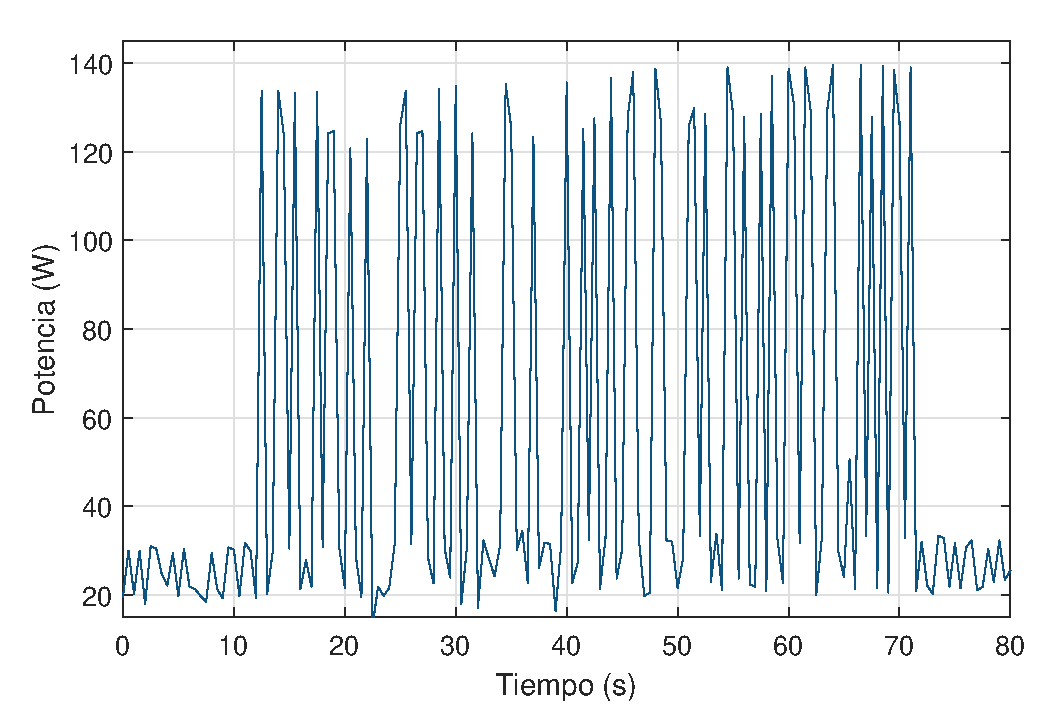
\includegraphics[scale=0.65]{Figuras/Exp3_P.eps}
\caption{Gráfico Potencia vs tiempo para el Experimento 4}
Fuente: Elaboración Propia
\label{exp3_P}
\end{figure}

\subsection{Análisis de Resultados:}

De los datos mostrados anteriormente se obtienen las siguientes conclusiones:

\begin{enumerate}
    \item Se comprueba la hipótesis de la relación existente entre el tamaño del paquete, el tiempo entre paquetes y la temperatura alcanzada por el módulo de potencia.
    
    \item Gracias a los experimentos se determinó que la causa del fallo en las transmisiones que se atribuían al radio, se debía a un daño y a la mala selección en la fuente de poder, ya que las corrientes las cuales no se muestran en este caso, excedían la capacidad de la fuente utilizada, y no se debía al circuito de protección como se pensaba, el cual se determinó en el manual que su función no es apagar el radio, sino más bien, si el mismo se encontraba en máxima potencia, el circuito, luego de cierta temperatura (la cual nunca se especifíca en el manual), bajará automáticamente el radio a la potencia mínima. Esto descarta la hipótesis que se tenía al inicio de este proyecto la cual supone que el calentamiento provocaba fallos en el radio.
    
    \item En ninguno de los cuatro casos se supera el límite de temperatura de 100\degree C establecido en el datasheet del módulo de potencia, el Experimento 1 el más cercano a este punto. Sin embargo, existen dos aspectos a considerar; el primero es que el Experimento 1 establece parámetros restrictivos de transmisión para el radio, es decir utilizar dichos parámetros u otros que representen un mayor esfuerzo térmico para el radio, podrían implicar degradación térmica de los componentes del módulo de potencia; por otra parte se debe aclarar que el límite de 100\degree C es especifico del módulo, mientras que el rango de operación máximo del radio de 60\degree C hace referencia a las condiciones generales y ambientales operativas del radio y dichos límites se deben considerar dentro los respectivos contextos.
    
    \item En la Figura \ref{comparacion} se muestra el gráfico comparativo de las temperaturas obtenidas en los cuatro experimentos, en donde se observa como la pendiente o bien el comportamiento de la curva varia con el tiempo entre paquetes y con el tamaño del paquete. Los cuatro experimentos plantean condiciones límites de parámetros de transmisión, ya que como se observa se debe tener un equilibrio entre el tamaño del paquete y el tiempo entre tramas o paquetes para lograr un perfil térmico de manera tal, que se pueda enviar la mayor cantidad de información dentro de los tiempos promedio de transmisión.
    
     \item La hipótesis inicial plantea que dentro de los valores mostrados en la Tabla \ref{parametros_experimento} se establecieron los tiempos entre paquetes; sin embargo al observar detenidamente los valores de potencia obtenidos en los experimentos se observa que el tiempo ingresado como parámetro es en realidad el tiempo de ciclo de trabajo que comprende tanto el tiempo de envió como el tiempo de delay entre paquetes.
    \item Del mismo análisis de la señal de potencia, se observa que existen irregularidades en los tiempos de transmisión para los experimentos 3 y 4, ya que se debe recordar, que aún cuando el paquete sea una línea de información, esto no quiere decir que se trate de una trama, con lo que se comprueba que internamente el radio segmenta la información de manera que para estos casos en específico se dificulta la identificación de un patrón; sin embargo dichos experimentos siguen representando el mejor perfil de transmisión para el radio desde una perspectiva térmica.
 
\end{enumerate}

\begin{figure}[H]
\centering
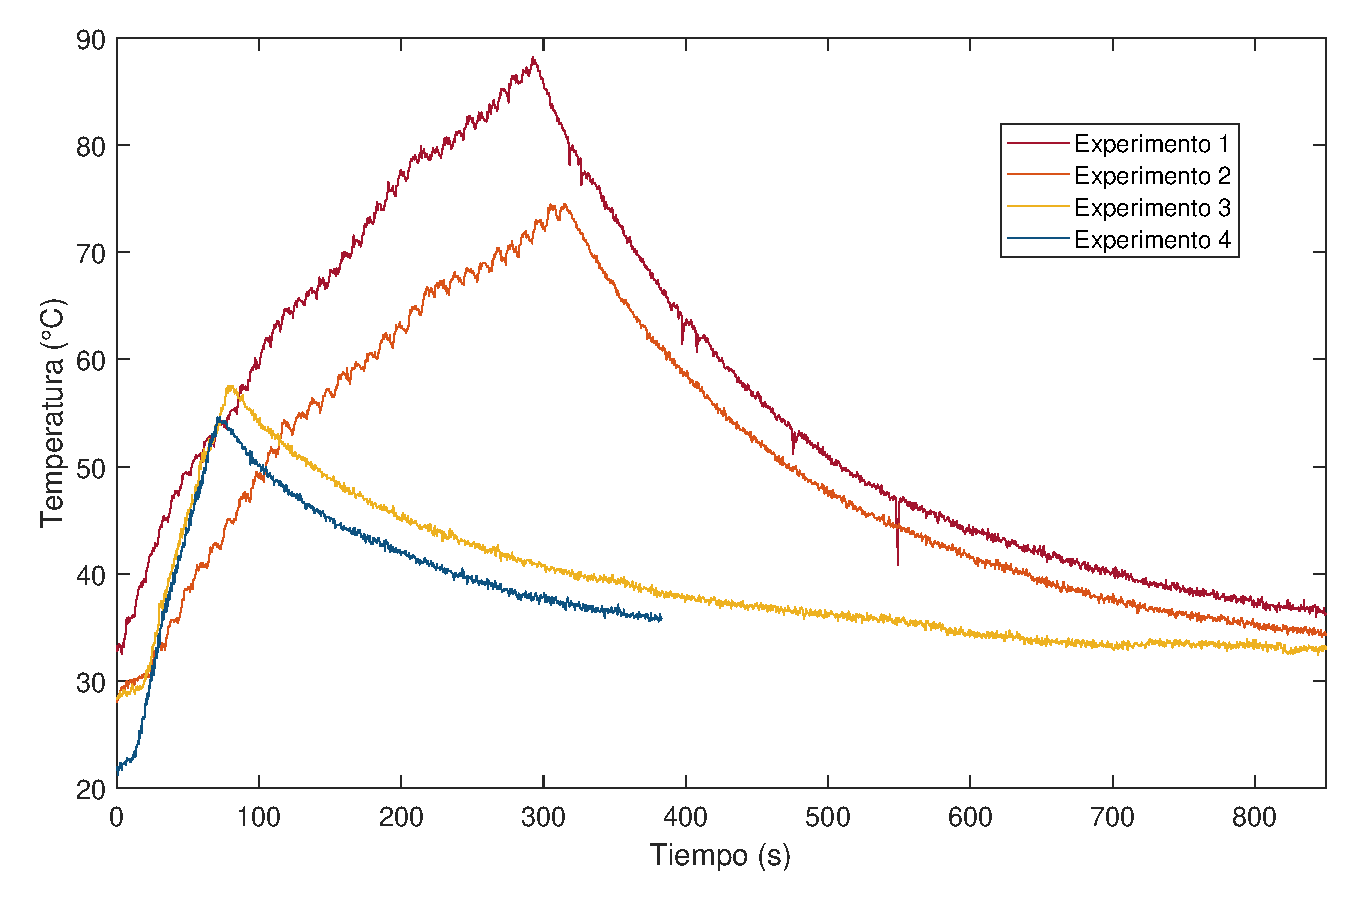
\includegraphics[width=\linewidth]{Figuras/comparacion.eps}
\caption{Gráfico Potencia vs tiempo para el Experimento 4}
Fuente: Elaboración Propia
\label{comparacion}
\end{figure}

Por otra parte en los Anexos \ref{anexo12},\ref{anexo13},\ref{anexo14},\ref{anexo15} se presentan parte del montaje utilizado para la realización de los experimentos.

\newpage
\section{Modelo Térmico del Radio}

Después de realizar el análisis respectivo de los datos obtenidos de los experimentos, se requería correlacionar los datos de potencia con el comportamiento térmico del radio; por lo que se recurrió a las herramientas de Matlab y Simulink para la implementación de una función de transferencia que relacione estas dos variables y en conjunto con la simulación de parámetros térmicos, se pueda obtener el perfil de temperatura obtenido en los experimentos; para lo cual se plantea el esquema de modelado de la Figura \ref{esquema_modelo_radio}. 

\begin{figure}[H]
\centering
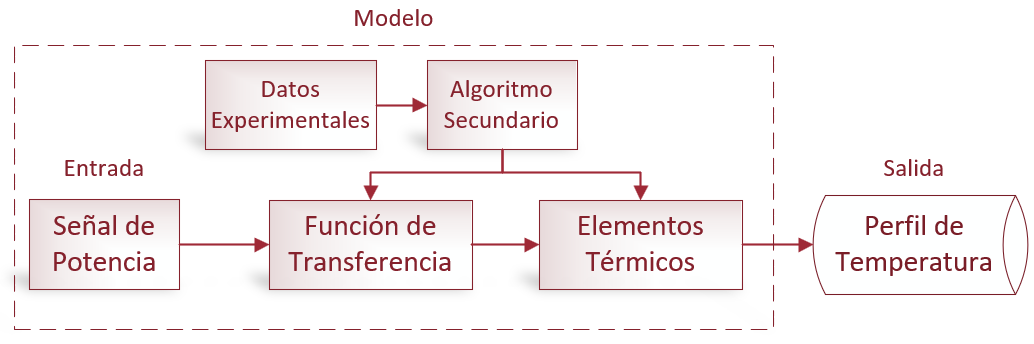
\includegraphics[scale=0.52]{Figuras/esquema_modelo_radio.png}
\caption{Esquema de modelo para el radio transmisor}
Fuente: Elaboración Propia
\label{esquema_modelo_radio}
\end{figure}

 A continuación se explica brevemente en que consiste cada bloque del esquema de modelado.
 
 \begin{itemize}
     \item \textbf{Datos Experimentales:} Son la base del modelo, ya que con esta información se obtendrán los datos del flujo de calor generado por el radio y establece a través de herramientas matemáticas la relación potencia-temperatura. Se seleccionaron los datos del experimento 2 para la elaboración del modelo debido a la homogeneidad en los datos de potencia; además los datos del experimento 1 representan un caso de parámetros límites de transmisión para el radio, por lo que para efectos del diseño son datos no deseables.
     \item \textbf{Algoritmo Secundario:} Comprende toda la parte de programación y cálculos que dan soporte a la función de transferencia y a los elementos de programación que simulan el comportamiento térmico; en este punto es de donde se determina la función de transferencia, para este caso se utiliza la función predeterminada de matlab \textit{tfest(data, np, nz)}, donde $np$ es la cantidad de polos y $nz$ es la cantidad de ceros.
     \item \textbf{Función de transferencia:} Hace referencia a su aplicación; se utilizó un número de polos de 5 y por ende 4 ceros. Su trabajo  es recibir los pulsos o señal de potencia eléctrica y convertirlos en un nivel de flujo de calor en un comportamiento determinado por la función misma.
     \item \textbf{Señal de Potencia:} Es la parte encargada de simular el comportamiento real de los pulsos de potencia eléctrica observados durante los experimentos y asociarlos a parámetros como tiempo de transmisión, tiempo entre paquetes, valor de potencia tanto en trasmisión como en reposo,entre otros; de manera tal que por medio de este bloque se pueda estimar el comportamiento térmico del radio al considerar diferentes parámetros de envió de datos. Este bloque a su vez representa una entrada virtual del modelo.
     \item \textbf{Elementos Térmicos:} Corresponde específicamente a la forma en que el software interpreta los diferentes mecanismos de transferencia de calor y los interconecta y relaciona matemáticamente con los demás elementos que conforman el modelo. 
     \item \textbf{Perfil de temperaturas:} Representa la salida del modelo, el cual luego de procesar la entrada, arroja como resultado el perfil de temperaturas asociado a los parámetros de potencia introducidos.
 \end{itemize}
 
En los Anexos \ref{anexo7} y \ref{anexo8} se muestra el algoritmo que se utilizó para simular el comportamiento de radio. En la Figura \ref{fit} se muestran los resultados superpuestos entre los datos experimentales y la curva de mejor ajuste obtenida mediante la función de transferencia, la cual tiene una aproximación de los datos reales en un \SI{96,18}{\percent} cuando se comparan los flujos de calor obtenidos del experimento 2.

\begin{figure}[H]
\centering
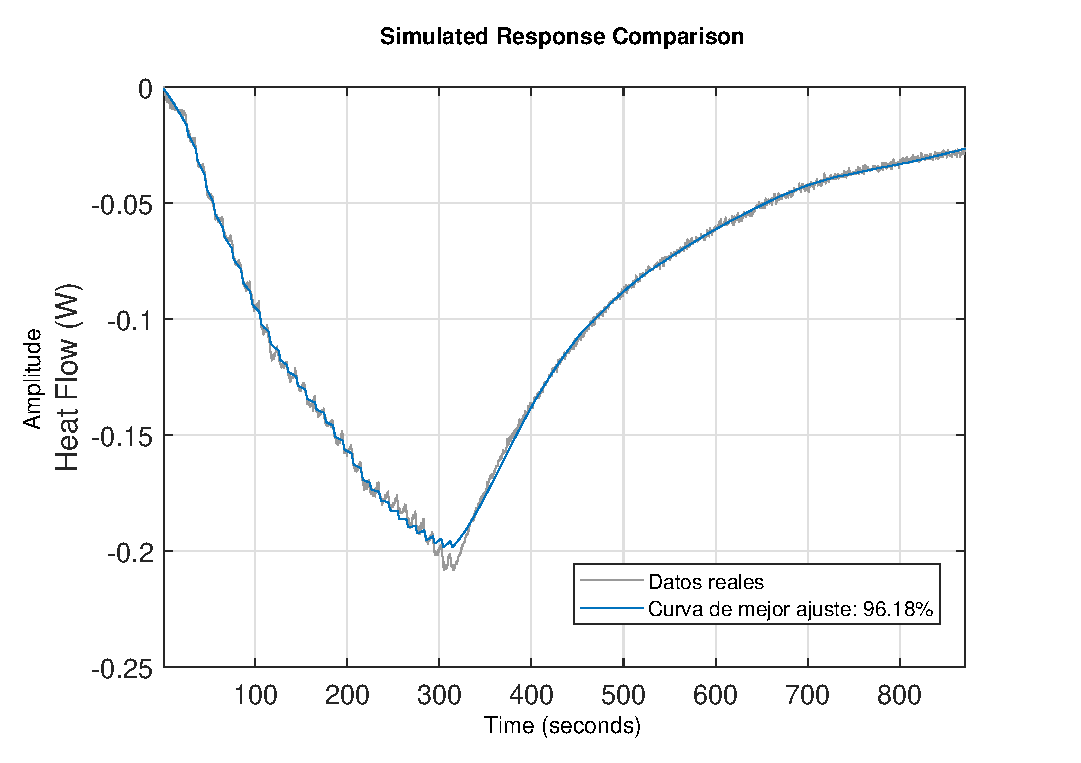
\includegraphics[scale=0.70]{Figuras/Fit.eps}
\caption{Gráfico comparativo entre los datos experimentales y la curva de mejor ajuste}
Fuente: Elaboración Propia
\label{fit}
\end{figure}

Para realizar los cálculos del flujo de calor se partió de la Ecuación \ref{Newton}, modelando la situación del radio en los experimentos como convección natural en entre la placa del módulo y el aire circundante, para lo cual se utilizaron los datos mostrados en la Tabla \ref{datosflujo}

\begin{table}[H]
\centering
\caption{Datos utilizados en la determinación del flujo de calor}
\label{datosflujo}
\begin{tabular}{lc}
\toprule
$h$ (\si{\watt/\meter\squared\celsius}) & 5 \\ % Mejor \SI{}{\watt/\meter\squared\degree} 
Área modulo (\si{\meter\squared}) & $8,964\times 10^{-4}$ \\ \bottomrule
\end{tabular}
\end{table}

La determinación del coeficiente de convección se establece a partir de la información en la literatura para convección natural \cite{redfrio}; más adelante para el modelo completo de la estación y considerando la posición del módulo de potencia, se realizará un cálculo más preciso de este coeficiente. La razón para determinar la tasa de transferencia de calor al considerar la convección natural radica en no entrar en complejidades técnicas y matemáticas al modelar el MOSFET de potencia desde su capas constructivas, máxime que el datasheet del módulo no contaba con la información suficiente para realizar dicha tarea, y si bien es cierto el módulo es el principal objeto de estudios de este proyecto, las acciones que se pueden realizar sobre el mismo no son internas, no pueden y no deben afectar de ninguna manera aspectos constructivos del módulo; por lo que para efectos de este proyecto es de interés la temperatura superficial que el mismo puede llegar a tener.

\begin{figure}[H]
\centering
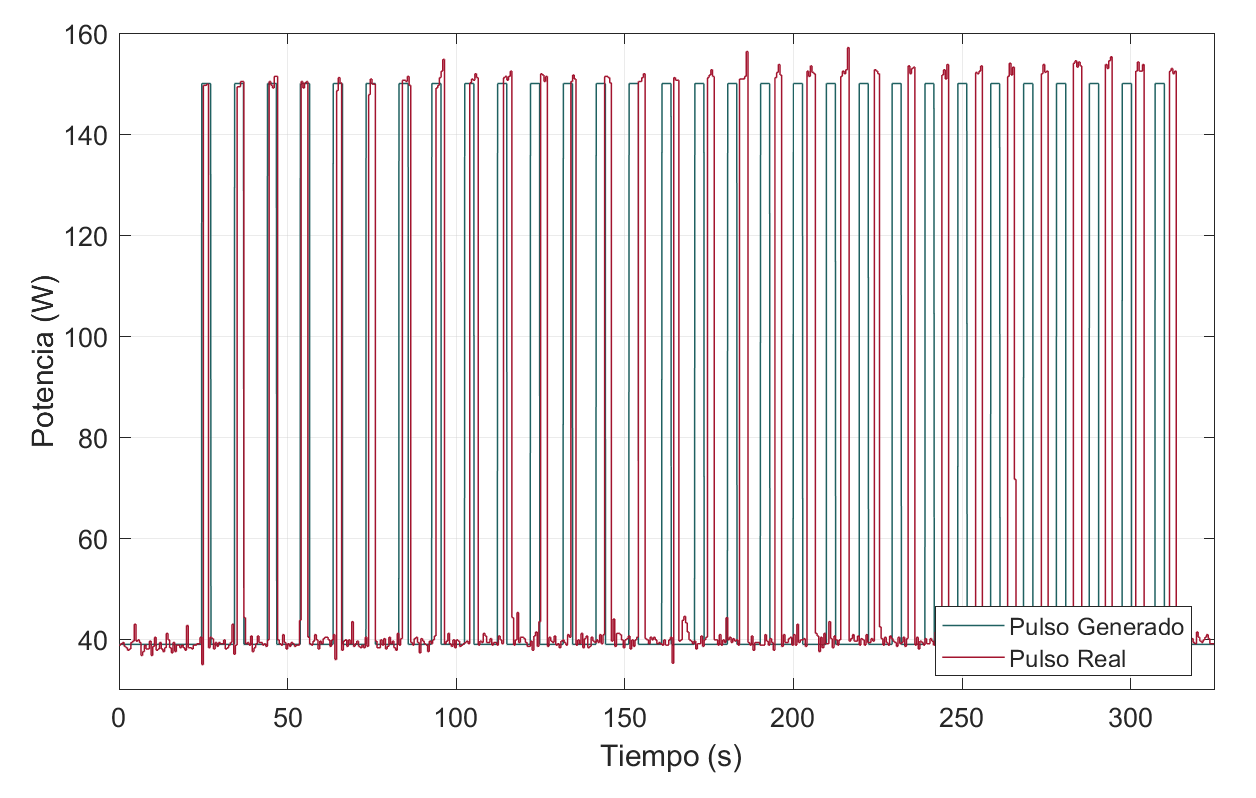
\includegraphics[scale=0.63]{Figuras/Resultado_P.eps}
\caption{Gráfico Potencia vs Tiempo para los resultados del modelado}
Fuente: Elaboración Propia
\label{resultado_P}
\end{figure}

\begin{figure}[H]
\centering
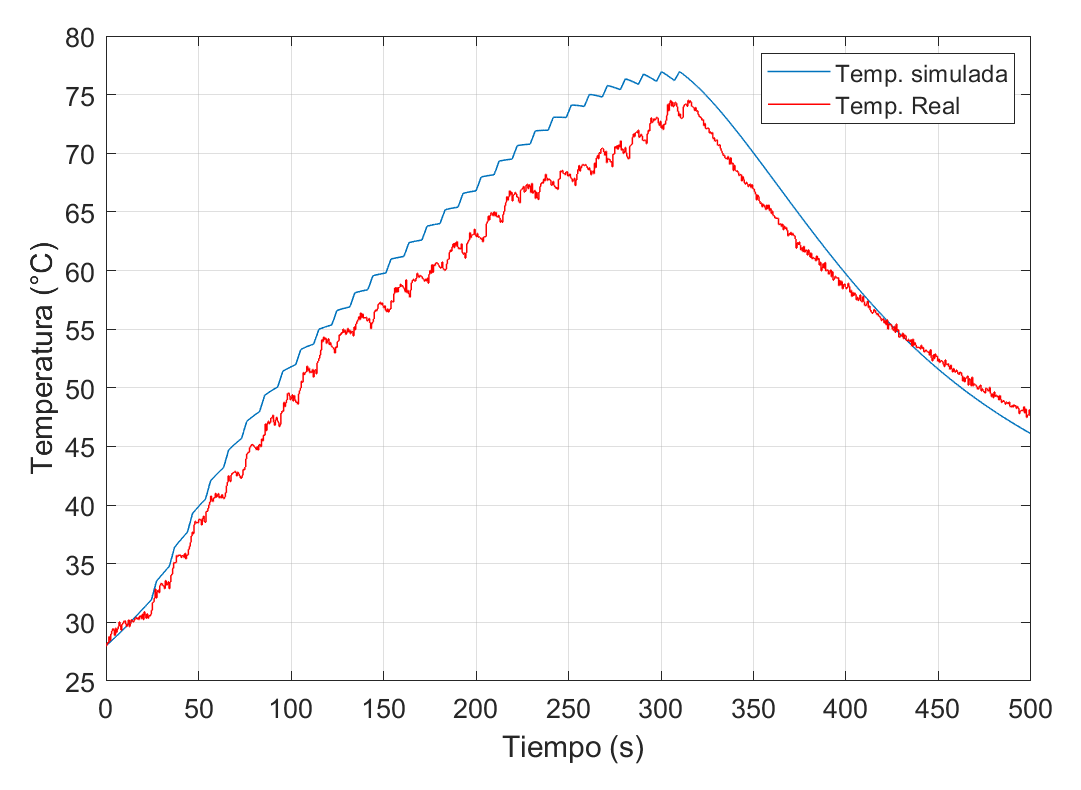
\includegraphics[scale=0.66]{Figuras/Resultado_T.eps}
\caption{Gráfico Temperatura vs Tiempo para los resultados del modelado}
Fuente: Elaboración Propia
\label{resultado_T}
\end{figure}

\begin{figure}[H]
\centering
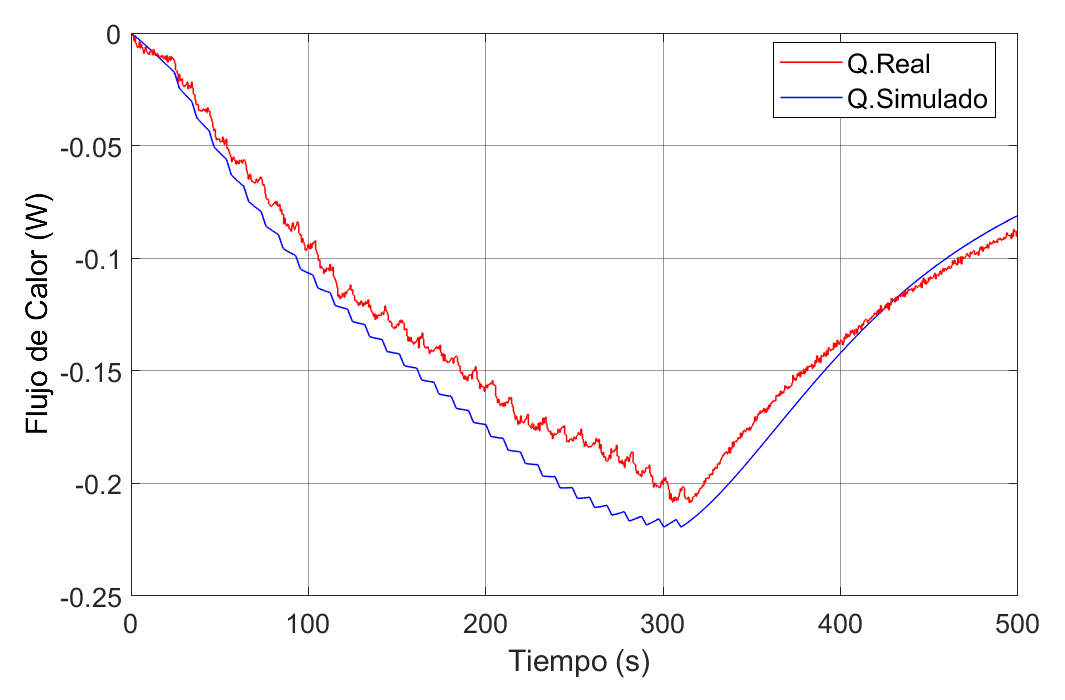
\includegraphics[scale=0.75]{Figuras/Resultado_Q.eps}
\caption{Gráfico Flujo de Calor vs Tiempo para los resultados del modelado}
Fuente: Elaboración Propia
\label{resultado_Q}
\end{figure}

\subsection{Observaciones del Modelo}

De los resultando antes mostrados se logran extraer las siguientes observaciones.

\begin{enumerate}
    \item En la Figura \ref{resultado_P} se hace evidente la irregularidad en los pulsos de potencias emitidos por el radio; ya que, si bien es cierto los primeros pulsos coinciden a la perfección con los simulados y los obtenidos experimentalmente, al transcurrir los segundos empieza a marcase un desfase, seguido de un ligero incremento de la potencia. Esto demuestra que la forma en que el radio transmite la información no es de manera homogénea, ya que básicamente el pulso simulado es una onda cuadrada de parámetros específicos y constantes.
    \item En la Figura \ref{resultado_T} se observa como a pesar de lo expuesto en el punto anterior, el modelo realiza una buena proyección del comportamiento térmico del radio, además de captar de manera óptima el comportamiento de la curva tanto para las temperaturas como para el flujo de calor (Figura \ref{resultado_Q}).
    \item Las principales discrepancias entre los datos reales y los simulados en las temperaturas y en el flujo de calor, se observa que ocurren justamente en el momento en que se dan las diferencias de potencia entre el pulso generado y el pulso medido.
    \item La determinación del coeficiente de convección para este caso fue acertada para las condiciones en las que se realizaron los experimentos que determinaron el modelo.
\end{enumerate}

\section{Validación del Modelo }

Por ser un apartado fundamental del proyecto, el cual por si solo tiene funcionalidad descriptiva, se realizó una validación del modelo construido para el radio transmisor; para lo cual se introdujeron los parámetros de transmisión obtenidos en los experimentos 1 y 3, es decir, se sometió el modelo a la prueba de simular la salida obtenida de los datos experimentales, haciendo uso de la herramienta implementada y se obtuvieron los resultados que se muestran mas adelante, los cuales se subdividen en dos validaciones.

Para ambos casos se utilizaron los mismos datos de la Tabla \ref{datosflujo}, variando los parámetros de transmisión aproximados acorde con los datos usados en los experimentos .Vale la pena anticipar que al igual que en el caso de los resultados del modelo, las aproximaciones de las curvas de calor y de temperatura están acorde con la aproximación de los pulsos de potencia, lo cual se dificultaba principalmente en la primera validación donde se observa que se tiene una situación donde dichos pulsos presentan irregularidades a lo largo de la transmisión; a pesar de ello el modelo nuevamente muestra que puede realizar una buena aproximación del comportamiento térmico del radio, por lo cual es apto para ser implementado en diferentes procesos y etapas del diseño, no solo de este proyecto, sino también de la misión.

\subsection{Primera Validación}

\begin{figure}[H]
\centering
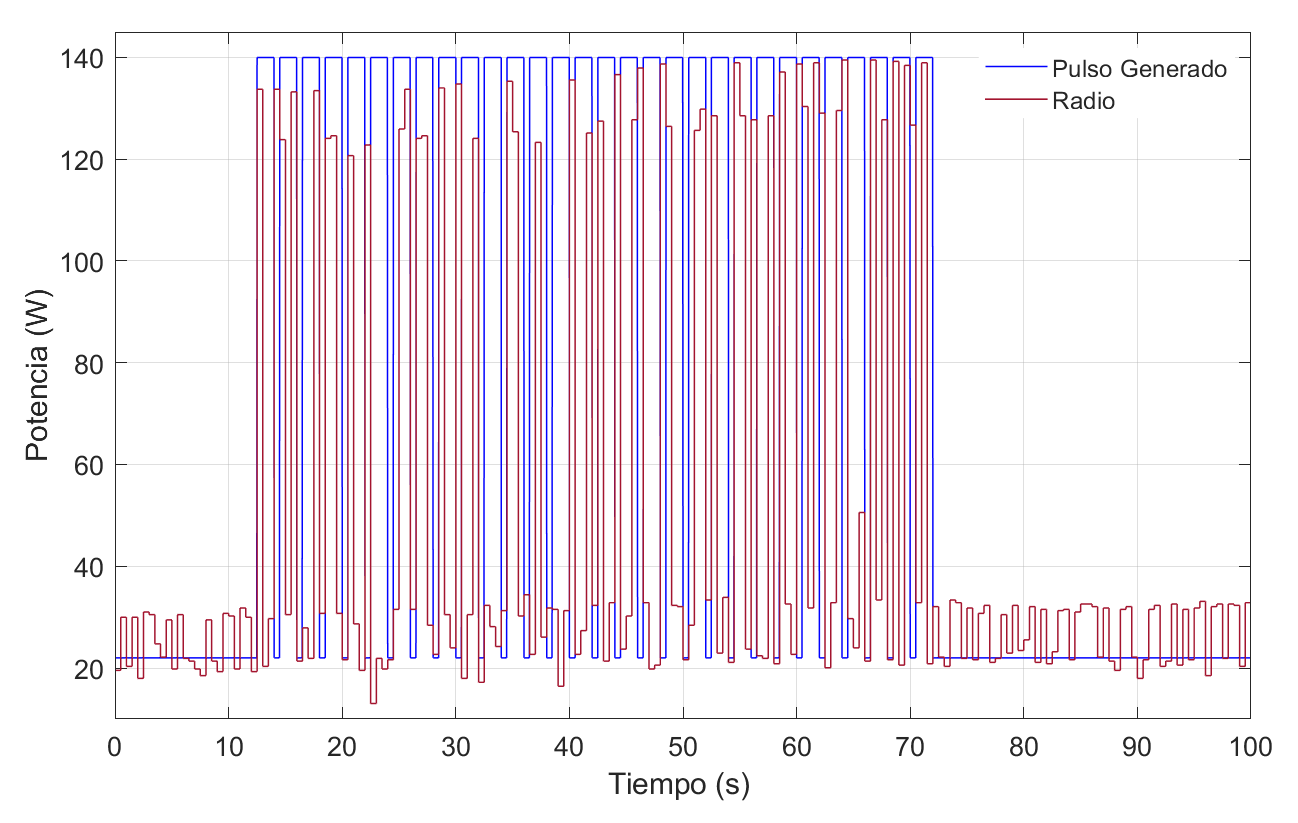
\includegraphics[scale=0.67]{Figuras/Validacion_1_P.eps}
\caption{Gráfico Potencias vs Tiempo de la primera validación}
Fuente: Elaboración Propia
\label{validacion_1_P}
\end{figure}

\begin{figure}[H]
\centering
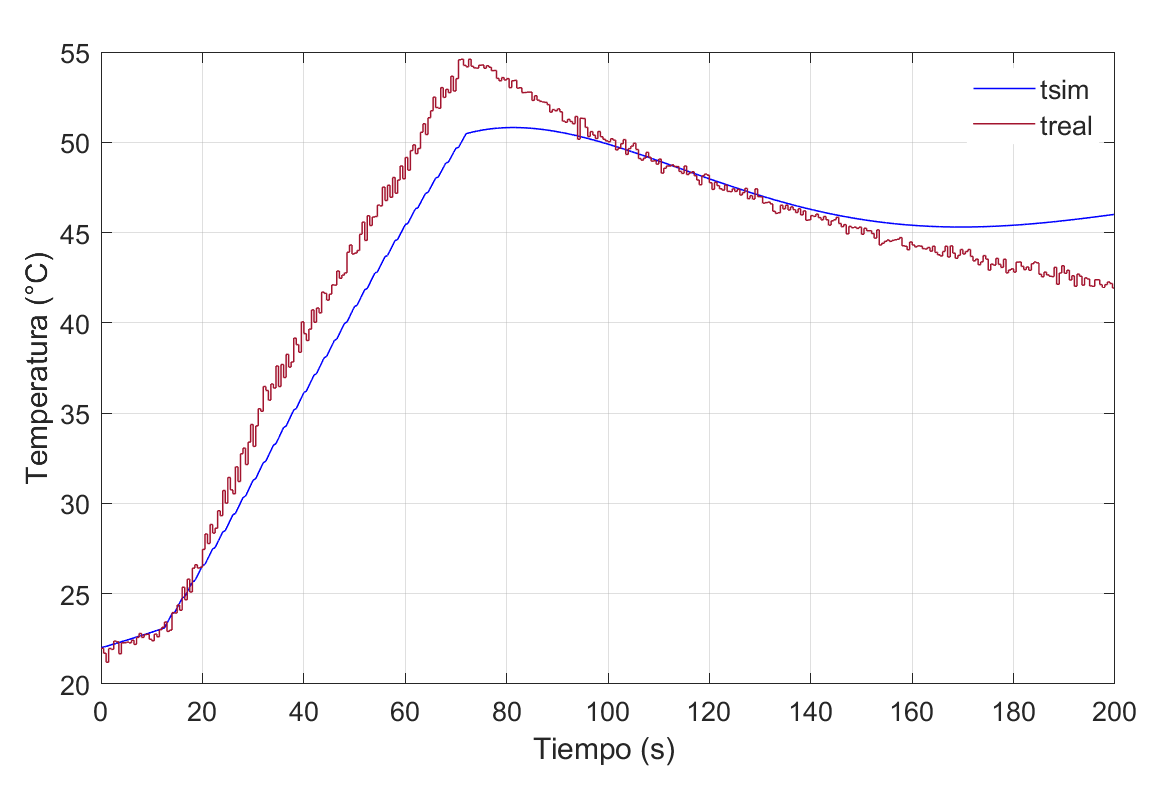
\includegraphics[scale=0.66]{Figuras/Validacion_1_T.eps}
\caption{Gráfico Temperaturas vs Tiempo de la primera validación}
Fuente: Elaboración Propia
\label{validacion_1_T}
\end{figure}

\begin{figure}[H]
\centering
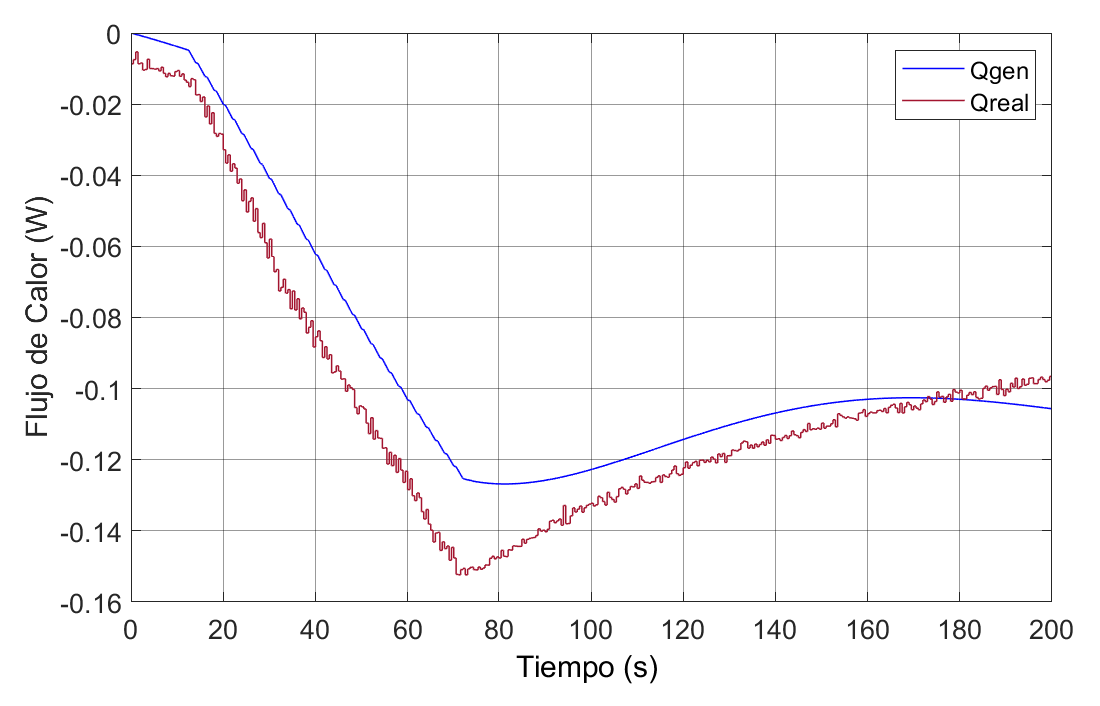
\includegraphics[scale=0.68]{Figuras/Validacion_1_Q.eps}
\caption{Gráfico Flujos de Calor vs Tiempo de la primera validación}
Fuente: Elaboración Propia
\label{validacion_1_Q}
\end{figure}

\subsection{Segunda validación}

\begin{figure}[H]
\centering
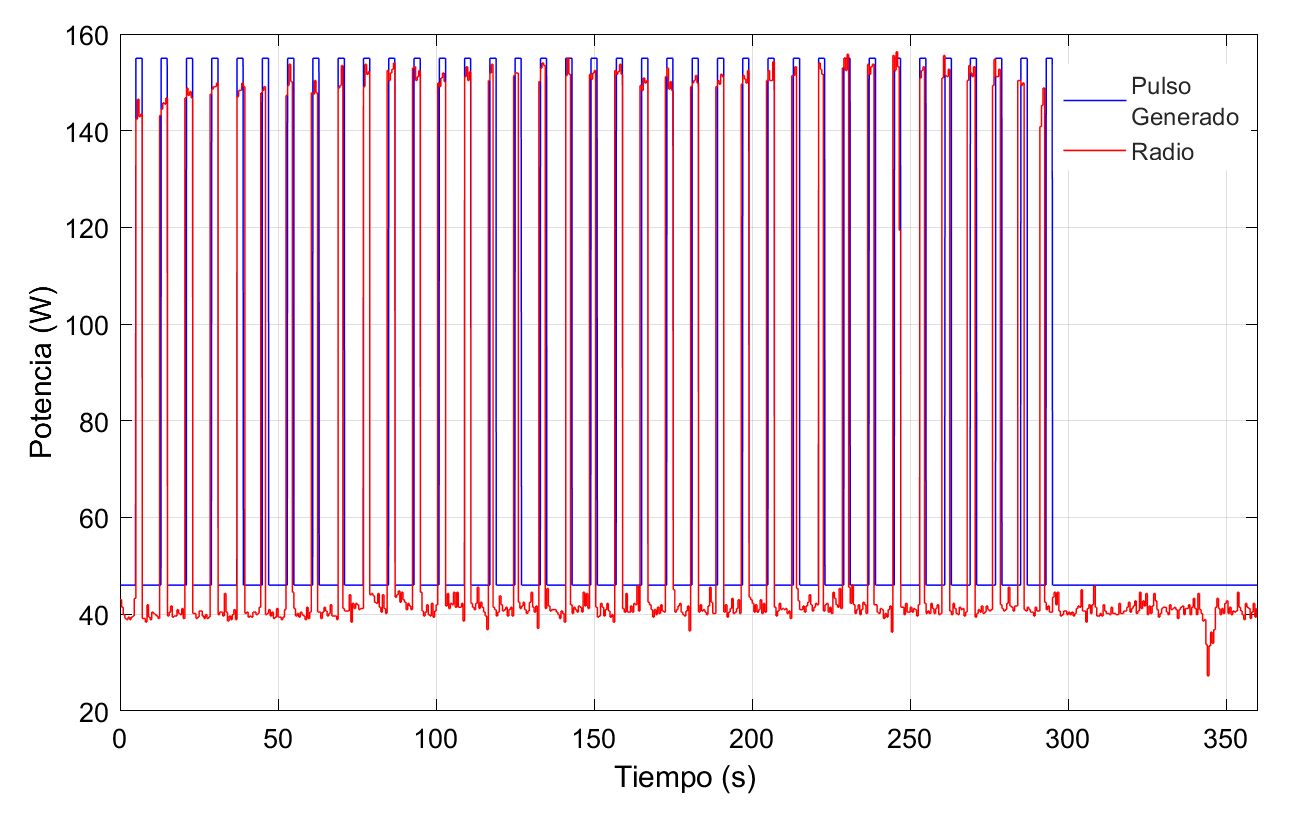
\includegraphics[scale=0.6]{Figuras/Validacion_2_P.eps}
\caption{Gráfico Potencias vs Tiempo de la segunda validación}
Fuente: Elaboración Propia
\label{validacion_2_P}
\end{figure}

\begin{figure}[H]
\centering
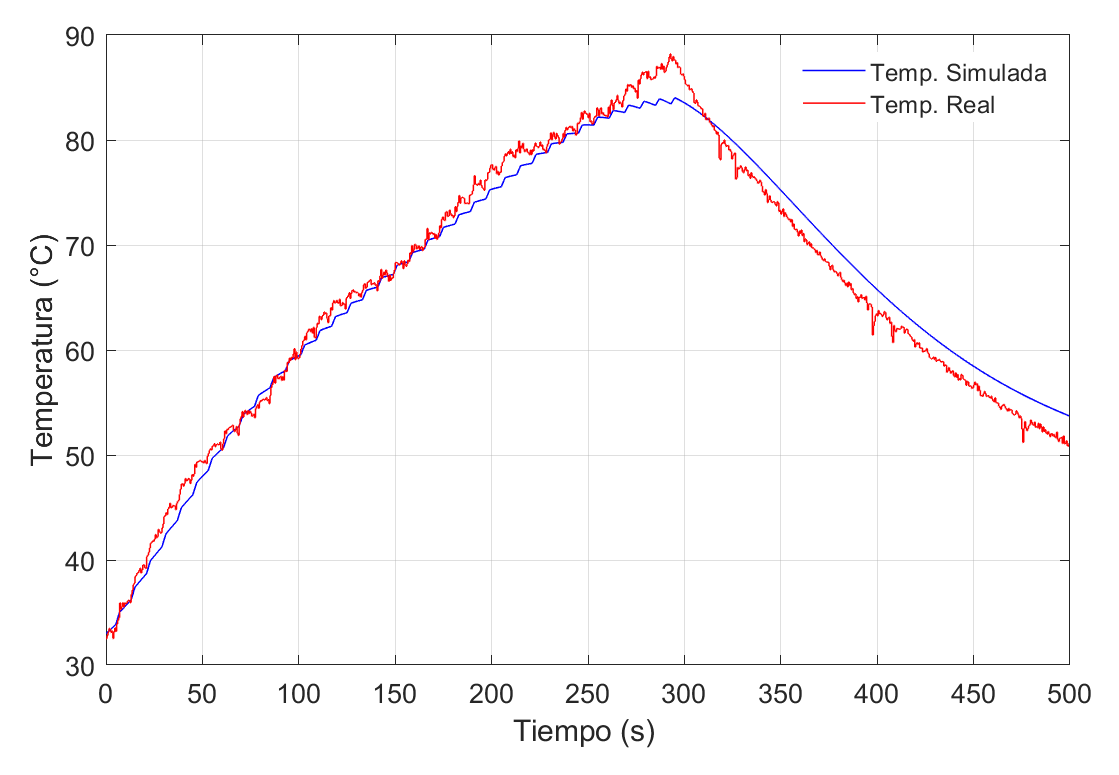
\includegraphics[scale=0.66]{Figuras/Validacion_2_T.eps}
\caption{Gráfico Temperaturas vs Tiempo de la segunda validación}
Fuente: Elaboración Propia
\label{validacion_2_T}
\end{figure}

\begin{figure}[H]
\centering
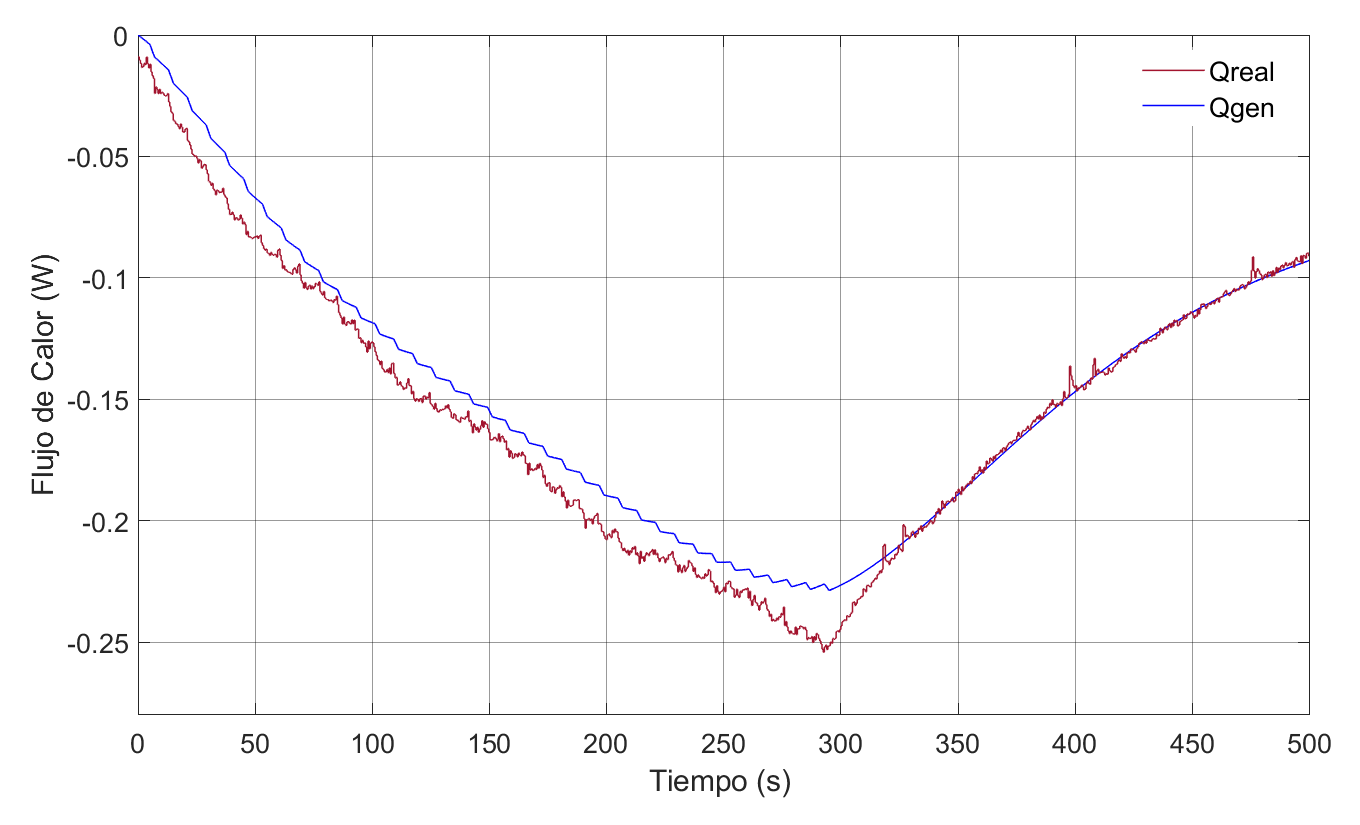
\includegraphics[scale=0.63]{Figuras/Validacion_2_Q.eps}
\caption{Gráfico Flujos de Calor vs Tiempo de la segunda validación}
Fuente: Elaboración Propia
\label{validacion_2_Q}
\end{figure}